\section{MRI physics} \label{sec:physics}

 {\Large Write top}
 
Magnetic resonance imaging (MRI) is founded on the principle of nuclear magnetic resonance (NMR), which exploits the magnetic properties of the hydrogen nucleus that contains a single proton. The proton is not static, but rotates around its own axis. As the proton is positively charged it creates a magnetic moment in the direction described by the thumb rule, and can interact with an external magnetic field. The human body consists of approximately 10\% hydrogen atoms, but as the hydrogen nuclei spins are randomly orientated, the net magnetic moment equals zero, as the nuclei cancel each other out. Placing the body in a strong magnetic field will align the nuclei. A property of the hydrogen nucleus is its quantum spin rate, which can either be $ \frac{1}{2}$ or $- \frac{1}{2}$ - either in the direction or the opposite direction of the main magnetic field. Most will align in the direction of the magnetic field, while some align in the opposite direction, possibly as a result of heat radiation absorbed by the nuclei. The direction of the nucleus is determined by its energy level, leaving the former in a low energy state and the latter in a high energy state. The nuclei do not simply point in the in the direction or opposite the direction of the magnetic field, but precess. \cite{Bharath2008} The rate of precession can be calculated by the Lamour frequency:
\begin{equation} \label{eq:lamour}
f=y*B_0
\end{equation} 
, where $f$ is precession frequency, $y$ is gyroscopic ratio and $B_0$ is magnetic field strength. The equation states that the precession frequency is proportional to the strength of the magnetic field. After canceling out all opposing precessing nuclei, the net magnetization, or longitudinal magnetization, will point in the direction of the external magnetic field. However, the longitudinal magnetization can not be detected directly as it points in the direction of the strong external magnetic field. Additional techniques are therefore used in NMR, to facilitate a detectable signal. \cite{Bharath2008} A depiction of how the nucleus precessing can either align along or opposite to the magnetic field depending on its energy state, can be found in \figref{fig:back:nucleus_precess}.  \\

\begin{figure}[H]                 
	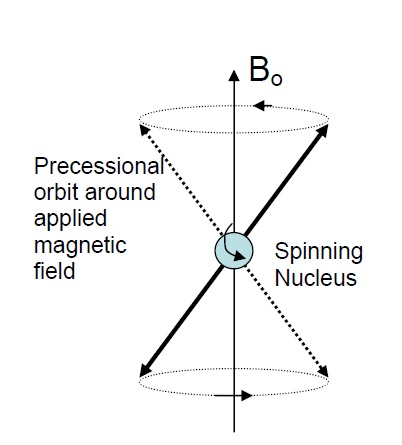
\includegraphics[width=.375\textwidth]{figures/aBackground/nucleus_precess}  
	\caption{The figure illustrates how the nucleus precess and spin in relation to the applied magnetic field $B_0$ surrounding it. The vectors, indicating the precessing, can go opposite or along the magnetic field depending on the nucleus energy state. \cite{Edwards}}
	\label{fig:back:nucleus_precess} 
\end{figure}  
A radio frequency pulse (RF pulse) tuned to the precession of the nuclei is transmitted in the vicinity of the nuclei. The RF pulse is absorbed by the nuclei and more, favorably half of the targeted nuclei population, will enter the high energy state, leaving the longitudinal magnetization to equal zero. The number of nuclei that flip is determined by the amount of energy the RF pulse injects, and the nuclei only exchange energy efficiently if the frequency of the energy from the RF pulse matches the precession rate. The RF pulse furthermore shifts the precession of the nuclei into same phase angle, which creates resonance, and a net magnetization pointing 90$^\circ$ to the longitudinal magnetization. This magnetization is called the transverse magnetization. The coherent nuclei produce a radio signal, or free induction decay signal (FID signal), that can be detected by a radio antenna. 
After the RF pulse is removed, the nuclei will relax into baseline state. Firstly, the spins of the nuclei will repel each other, as they are positively charged, and thus shift phase. The net magnetization will return to zero. This relaxation is called $T_2$ or “spin-spin” relaxation, as the energy exchange between the nucleus spins is causing the relaxation. A second relaxation appears as the high energy nuclei returns to the low energy state. The energy that was previously absorbed by the nuclei is dissipated in to the surrounding lattice in the form of heat. During this relaxation the longitudinal magnetization is regrown. This relaxation is called $T_1$ or “spin-lattice” relaxation, as the spins transfer energy to the surrounding lattice. \cite{Bharath2008}
{\Large (Insert illustration)} \\
The hydrogen nuclei are located in different local environments in the body. Some are for instance associated with free-floating water molecules, while others are associated with structural and storage molecules such as proteins and lipids, and thus more fixed in position. The nuclei have different $T_1$ and $T_2$ relaxation characteristics, depending on the local environment or tissue they are associated with. This can be accentuated and measured in NMR. \cite{Bharath2008} \\
The chosen pulse sequence is key to how the tissue will be portrayed in an image, and is described by the $T_{echo}$, time before the FID signal is measured, and $T_{rep}$, time before a new RF pulse is applied. In a case of nuclei associated with lipids and water molecules, the nuclei in lipids are fixed and will have a fast $T_1$ relaxation after exposure to a RF pulse . Meanwhile the nuclei in the water molecules will maintain being in a synchronized phase. At $T_{echo}$, the nuclei associated with the lipids will have a low amplitude FID signal, as the transverse magnetization is weak, and the nuclei associated with the water molecules will have a high amplitude FID signal, as the transverse magnetization is strong. The water molecules will be assigned a white color on a greyscale image and the lipids as dark grey/black. In this case there is a long $T_{echo}$ and a long $T_{rep}$, and is referred to as $T_2$-weighted MRI. \cite{Bharath2008} \\
In case of $T_1$-weighted MRI, the $T_{echo}$ and $T_{rep}$ are short. As in $T_2$-weighted MRI a RF pulse is applied and the nuclei associated with lipids will quickly return to baseline state and the water molecule nuclei will remain a strong transverse magnetization. At this time point a second RF pulse will be induced, referring to the short $T_{rep}$. Now the lipid nuclei will return to a strong transverse magnetization state and excite a high FID signal. More low energy state nuclei of the water molecules will absorb the RF pulse and shift to a high energy state, leaving a majority of nuclei in a high energy state. The water molecule nuclei now has a weak transverse magnetization and 180 degrees longitudinal magnetization, thus producing a low-amplitude FID signal. A short $T_{echo}$ after the second RF pulse then shows lipids as white and the water molecules as dark grey/black in a greyscale image. \cite{Bharath2008} 

Additionally to $T1$ and $T2$, another relaxation occur called $T2^*$. During the transverse relaxation, irreversible dephasing of the transverse magnetization is caused. But there is also a reversible dephasing happening, which is caused by local and global magnetic field inhomogeneities. This reversible dephasing is called $T2^*$. To acquire a $T2^*$-weighted image, a gradient-echo sequence (GRE) is required, most of these are $T2^*$ sensitive. These do not use a $180^\circ$ flip to compensate for the magnetic field inhomogeneities. A longer TE introduces a greater signal loss and as the TE increases, so does $T2^*$ sensitivity as more dephasing occurs. Introducing a low flip angle reduces the $T1$ influence making the $T2^*$ dominant. \cite{Chavhan2009}  

